\documentclass{standalone}
\usepackage{tikz}
\usepackage{ctex,siunitx}
\usepackage{tkz-euclide}
\usepackage{amsmath}
\usetikzlibrary{patterns, calc}
\usetikzlibrary {decorations.pathmorphing, decorations.pathreplacing, decorations.shapes,}
\begin{document}
\small
\begin{tikzpicture}[>=latex,scale=1.0]
  \draw[->] (0,0)node[left]{$Q$}--(1,2)node[left]{$P$}--(1.5,3)node[above]{$E$};
  \draw (0,0) [fill=black] circle (1.5pt);
  \draw (1,2) [fill=black] circle (1.5pt);
  \end{tikzpicture}
  \qquad 	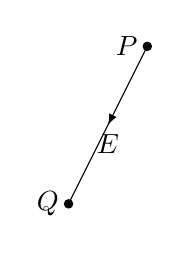
\begin{tikzpicture}[>=latex]
      \draw[->] (0,0)node[left]{$Q$}--(1,2)node[left]{$P$}--(.5,1)node[below]{$E$};
      \draw (0,0) [fill=black] circle (1.5pt);
  \draw (1,2) [fill=black] circle (1.5pt);
\end{tikzpicture}
\end{document}